
Historically, C++ started with supporting polymorphism only through the use of inheritance combined with virtual functions.

\begin{tcolorbox}[colback=webgreen!5!white,colframe=webgreen!75!black]
\hspace*{0.75cm}Strictly speaking, macros can also be thought of as an early form of static polymorphism. However, they are left out of consideration because they are mostly orthogonal to the other language mechanisms.
\end{tcolorbox}

The art of polymorphic design in this context consists of identifying a common set of capabilities among related object types and declaring them as virtual function interfaces in a common base class.

The poster child for this design approach is an application that manages geometric shapes and allows them to be rendered in some way (e.g., on a screen). In such an application, we might identify an abstract base class (ABC) GeoObj, which declares the common operations and properties applicable to geometric objects. Each concrete class for specific geometric objects then derives from GeoObj (see Figure 18.1):

\begin{center}
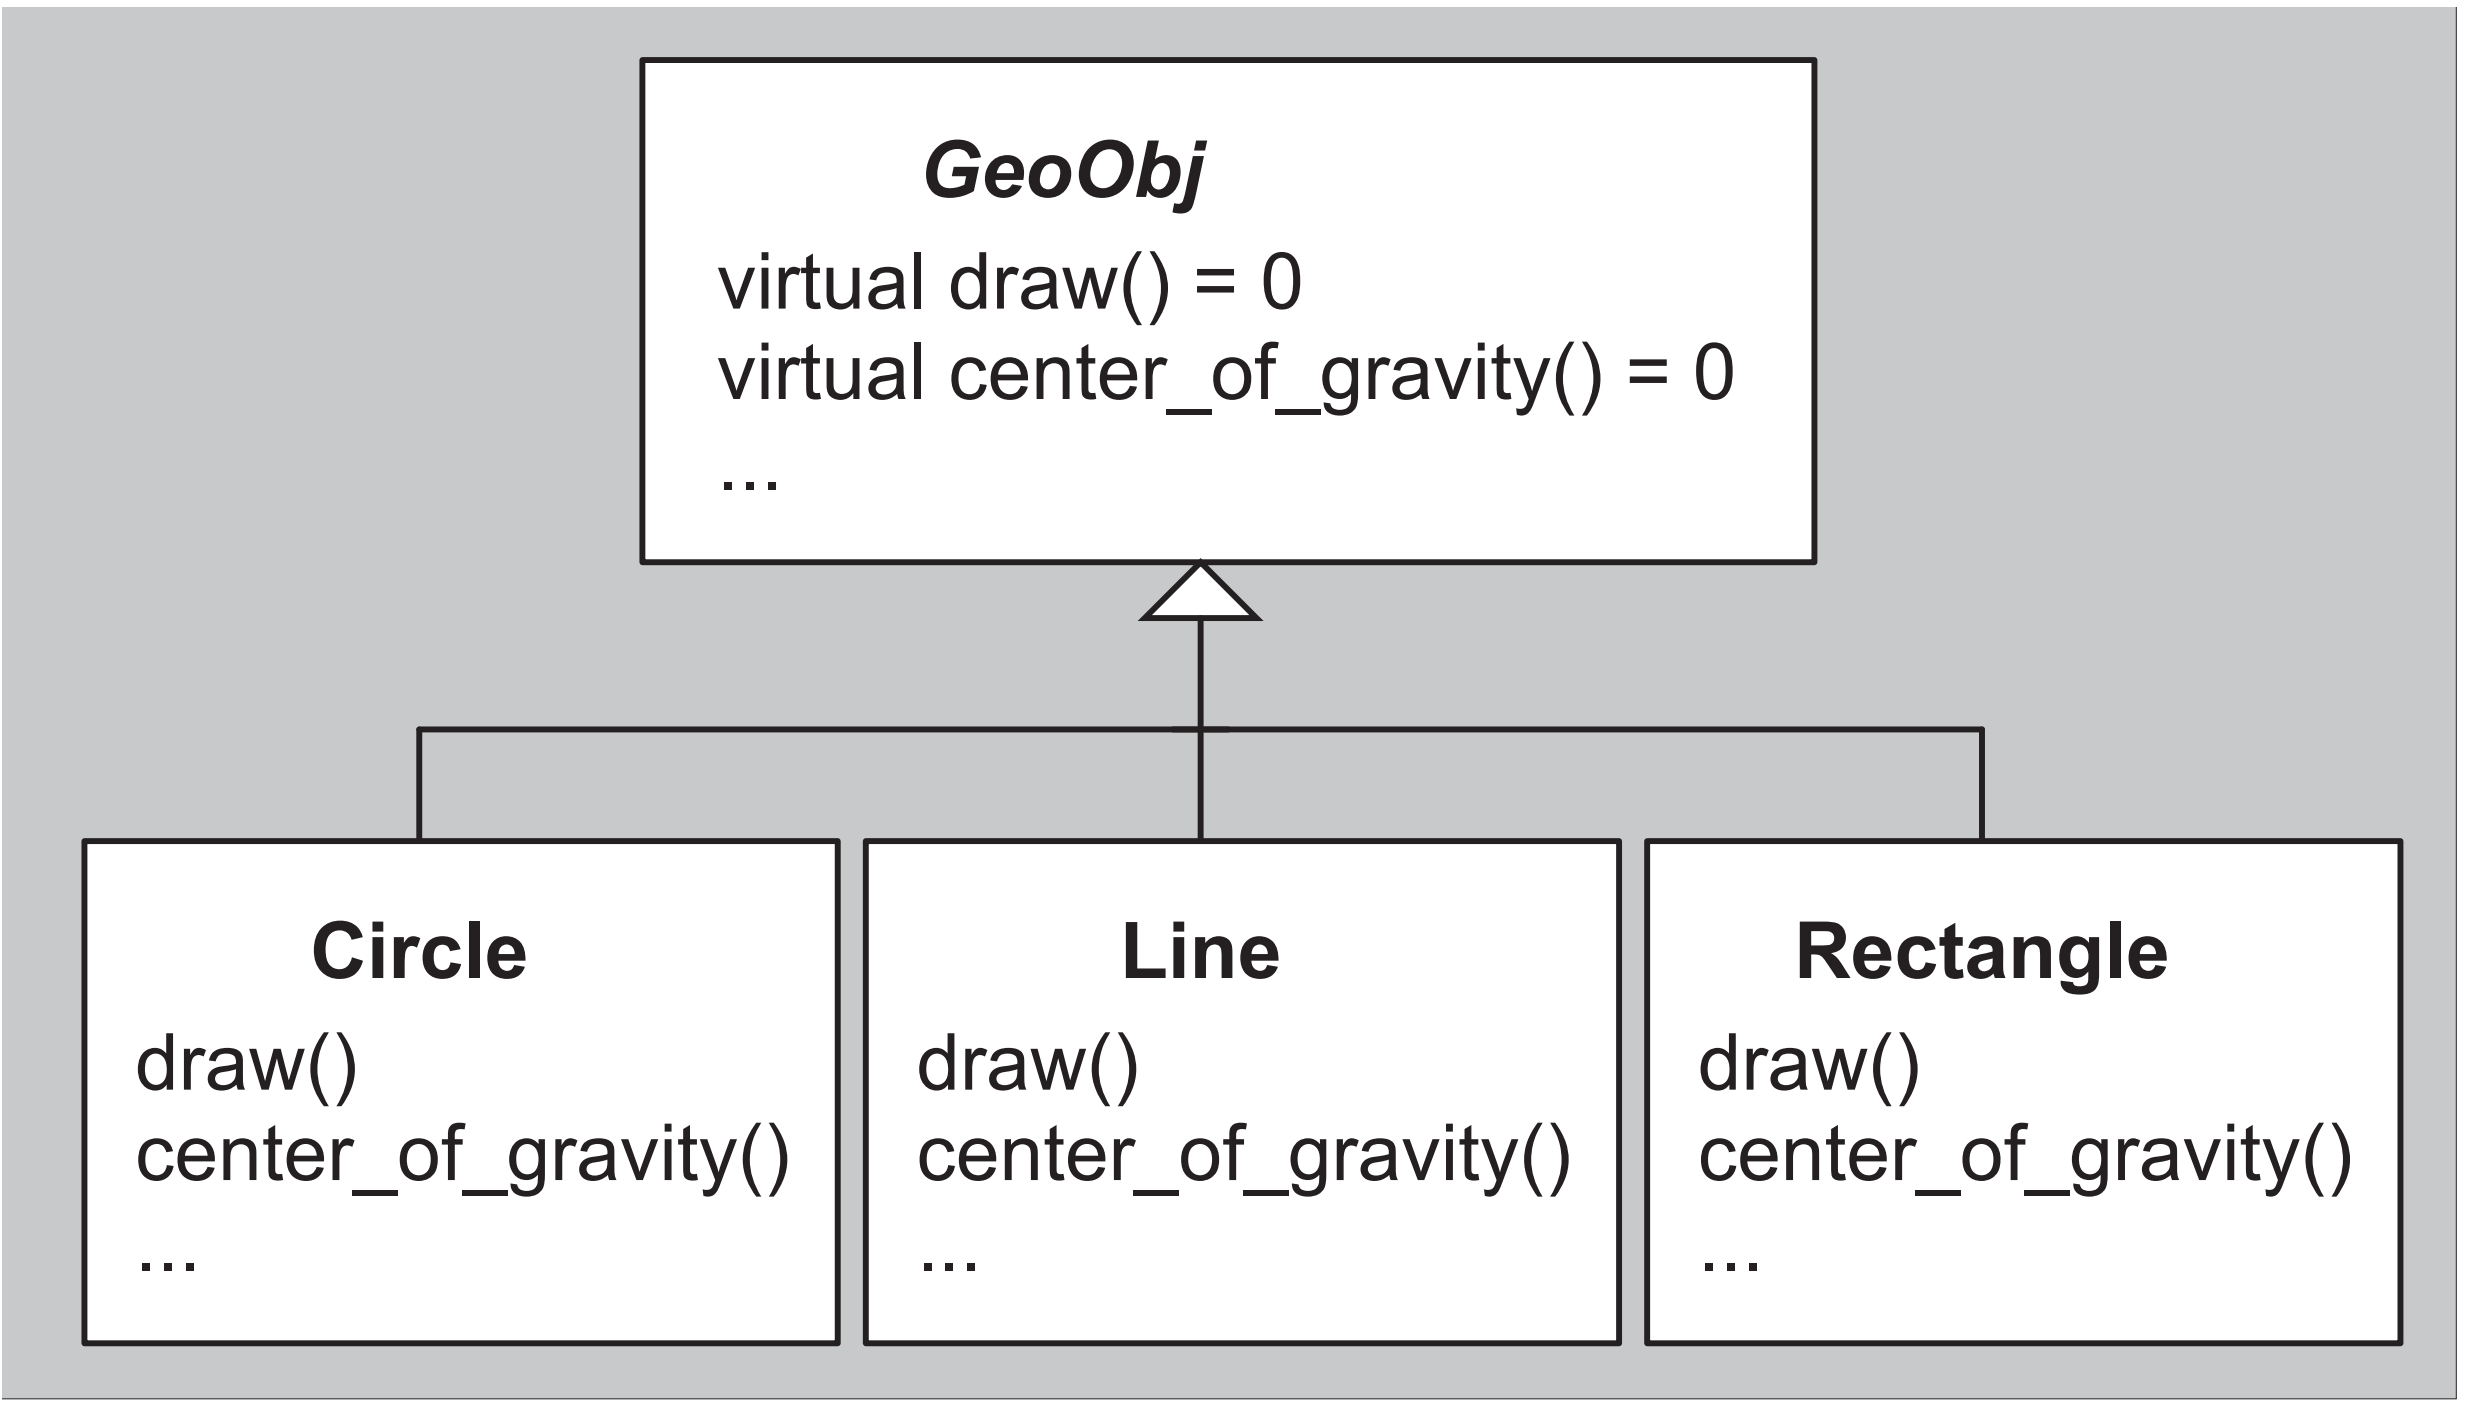
\includegraphics[width=0.8\textwidth]{content/3/chapter18/images/1.png} \\
Figure 18.1. Polymorphism implemented via inheritance
\end{center}

\hspace*{\fill} \\ %插入空行
\noindent
\textit{poly/dynahier.hpp}
\begin{lstlisting}[style=styleCXX]
#include "coord.hpp"

// common abstract base class GeoObj for geometric objects
class GeoObj {
	public:
	// draw geometric object:
	virtual void draw() const = 0;
	// return center of gravity of geometric object:
	virtual Coord center_of_gravity() const = 0;
	...
	virtual ~GeoObj() = default;
};

// concrete geometric object class Circle
// - derived from GeoObj
class Circle : public GeoObj {
	public:
	virtual void draw() const override;
	virtual Coord center_of_gravity() const override;
	...
};

// concrete geometric object class Line
// - derived from GeoObj
class Line : public GeoObj {
	public:
	virtual void draw() const override;
	virtual Coord center_of_gravity() const override;
	...
};
...
\end{lstlisting}

After creating concrete objects, client code can manipulate these objects through references or pointers to the common base class by using the virtual function dispatch mechanism. Calling a virtual member function through a pointer or reference to a base class subobject results in an invocation of the appropriate member of the specific (“most-derived”) concrete object being referred to.

In our example, the concrete code can be sketched as follows:

\hspace*{\fill} \\ %插入空行
\noindent
\textit{poly/dynapoly.hpp}
\begin{lstlisting}[style=styleCXX]
#include "dynahier.hpp"
#include <vector>

// draw any GeoObj
void myDraw (GeoObj const& obj)
{
	obj.draw(); // call draw() according to type of object
}

// compute distance of center of gravity between two GeoObjs
Coord distance (GeoObj const& x1, GeoObj const& x2)
{
	Coord c = x1.center_of_gravity() - x2.center_of_gravity();
	return c.abs(); // return coordinates as absolute values
}

// draw heterogeneous collection of GeoObjs
void drawElems (std::vector<GeoObj*> const& elems)
{
	for (std::size_type i=0; i<elems.size(); ++i) {
		elems[i]->draw(); // call draw() according to type of element
	}
}

int main()
{
	Line l;
	Circle c, c1, c2;
	
	myDraw(l); // myDraw(GeoObj&) => Line::draw()
	myDraw(c); // myDraw(GeoObj&) => Circle::draw()
	
	distance(c1,c2); // distance(GeoObj&,GeoObj&)
	distance(l,c); // distance(GeoObj&,GeoObj&)
	
	std::vector<GeoObj*> coll; // heterogeneous collection
	coll.push_back(&l); // insert line
	coll.push_back(&c); // insert circle
	drawElems(coll); // draw different kinds of GeoObjs
}
\end{lstlisting}

The key polymorphic interface elements are the functions draw() and center\_of\_gravity(). Both are virtual member functions. Our example demonstrates their use in the functions mydraw(), distance(), and drawElems(). The latter functions are expressed using the common base type GeoObj. A consequence of this approach is that it is generally unknown at compile time which version of draw() or center\_of\_gravity() must be called. However, at run time, the complete dynamic type of the objects for which the virtual functions are invoked is accessed to dispatch the function calls.

\begin{tcolorbox}[colback=webgreen!5!white,colframe=webgreen!75!black]
\hspace*{0.75cm}That is, the encoding of polymorphic base class subobjects includes some (mostly hidden) data that enables this run-time dispatch.
\end{tcolorbox}

Hence, depending on the actual type of a geometric object, the appropriate operation is performed: If mydraw() is called for a Line object, the expression obj.draw() calls Line::draw(), whereas for a Circle object, the function Circle::draw() is called. Similarly, with distance(), the member functions center\_of\_gravity() appropriate for the argument objects are called.

Perhaps the most compelling feature of this dynamic polymorphism is the ability to handle heterogeneous collections of objects. drawElems() illustrates this concept: The simple expression

\begin{lstlisting}[style=styleCXX]
elems[i]->draw()
\end{lstlisting}

results in invocations of different member functions, depending on the dynamic type of the element being iterated over.


























